\chapter{Evaluación Experimental}\label{chap:evaluacion}

En este capitulo se expondrá los resultados obtenidos de los experimentos realizados. El capítulo se dividirá en secciones diferentes para dar al lector una mayor compresión de los resultados.

La primera sección \textit{Preparación de Datos} \ref{sec:preparacion_de_datos}, se desarrolla cuales son los recursos que se utilizaron para realizar la experimentación.

La segunda sección  \textit{Entrenamiento y Validación} \ref{sec:entrenamiento}, se detallan como se realizo el proceso de aprendizaje de los datos y los procesos de validación que se llevaron a cabo; a su vez se detallan las métricas obtenidas de cada predictor entrenado.

\section{Preparación de Datos}\label{sec:preparacion_de_datos}

Vamos a partir de las imágenes obtenidas en el capitulo \ref{chap:recoleccion} donde se puso en detalle los tipos de imágenes que serán utilizadas. En esta sección hablaremos de cual es el \textit{ground truth}, región de interés utilizada; como se realizo la extracción de característica de cada imagen, y que criterio de selección de candidatos se utilizo para el entrenamiento.

\subsection{Ground truth}\label{sub:groundtruth}

El problema abordado es un problema de clasificación supervisada, es por esto que debemos saber anticipadamente donde se encuentra el objeto de interés que deseamos detectar. En \ac{ml} el termino \textit{ground truth} hace referencia a la información provenida desde la observación; \textit{ground truth} involucra a un conjunto de imágenes y un conjunto de etiquetas en las imágenes que incluye la locación y las características claves en la imagen.

Las etiquetas se añadieron manualmente utilizando una librería desarrollada en python llamada \textit{labelme}\footnote{Fuente: 
https://github.com/wkentaro/labelme}; que nos permite realizar las anotaciones de las zonas de interés sobre la imagen.

\begin{figure}[h]
 \centering
  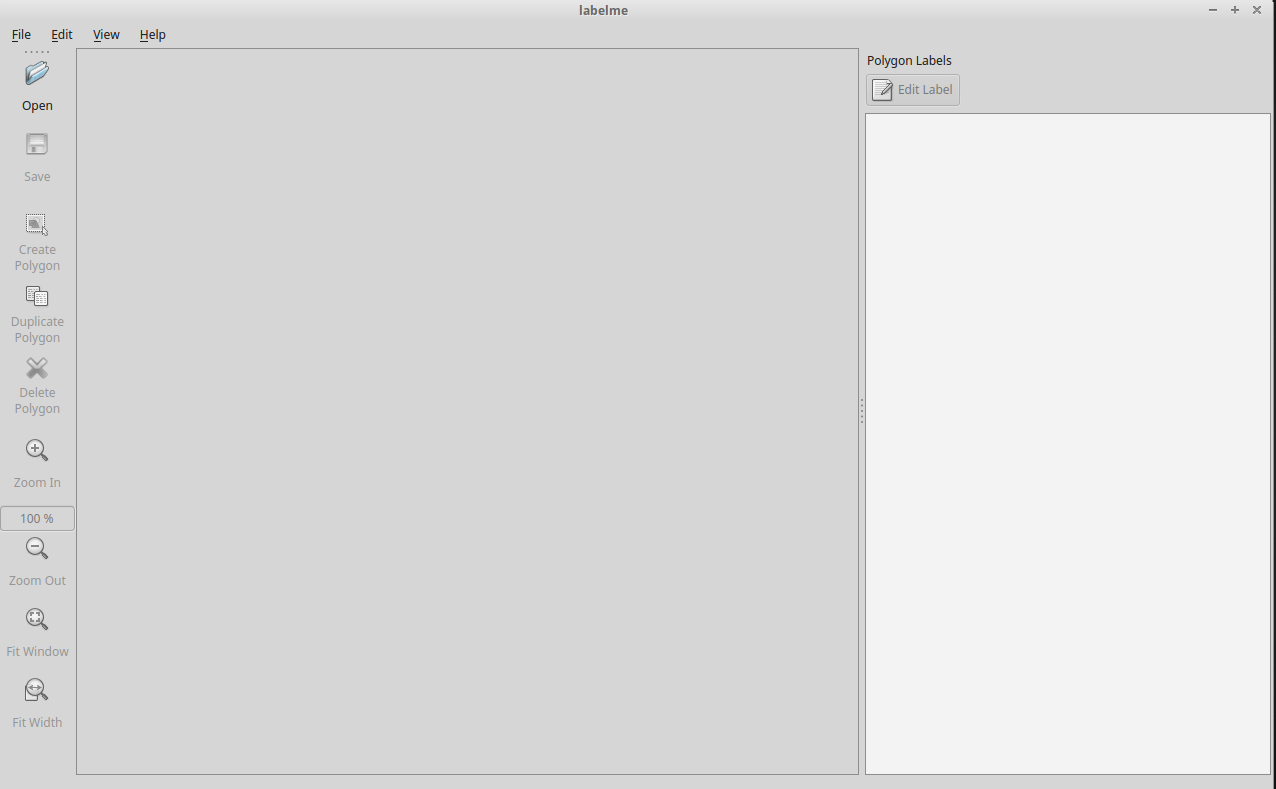
\includegraphics[height=9cm,keepaspectratio=true,clip=true]{imagenes/Logos/labelme.png}
  \caption{Pantalla Principal \textit{labelme}}
	\label{Fig: labelme}
\end{figure}

En las imágenes siguientes se muestra el proceso de anotación que se llevo a cabo mediante \textit{labelme}, para detalles de la instalación ir a: \ref{sec:instalacionlabelme}.

Cada anotación se almacena en un archivo .json que luego es transformado y almacenado en una tabla como vemos en \ref{tab:ejemGT}
\begin{figure}[h]
 \centering
  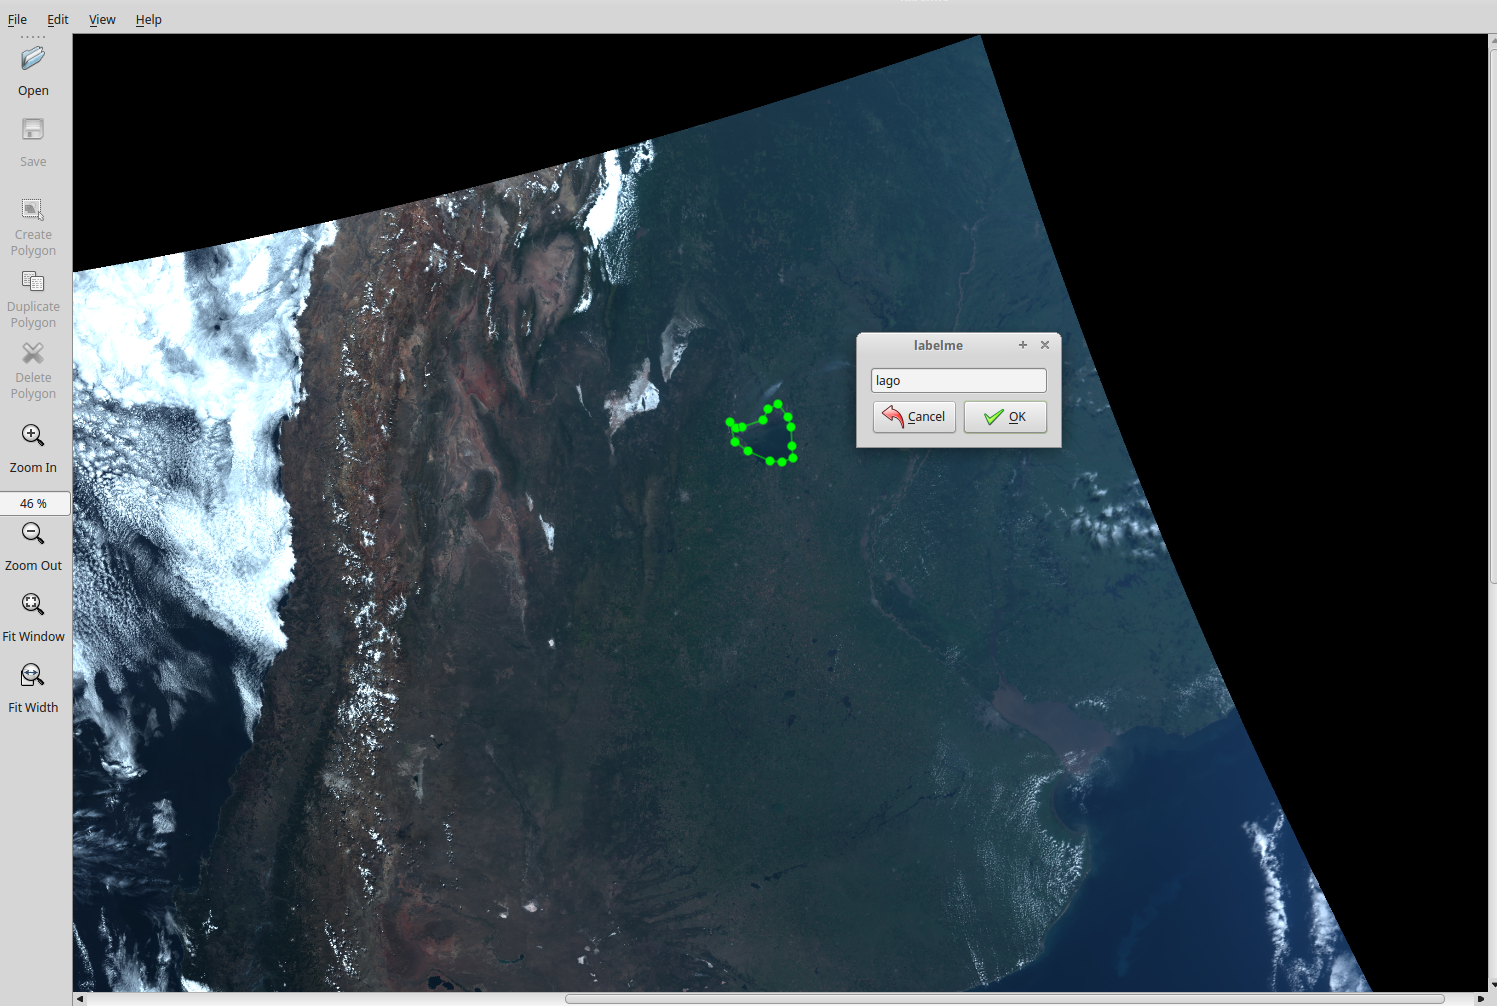
\includegraphics[height=8cm,keepaspectratio=true,clip=true]{imagenes/Logos/labelme1.png}
  \caption{Etiquetar una región en \textit{labelme}}
	\label{Fig: labelme1}
\end{figure}

\begin{figure}[H]
 \centering
  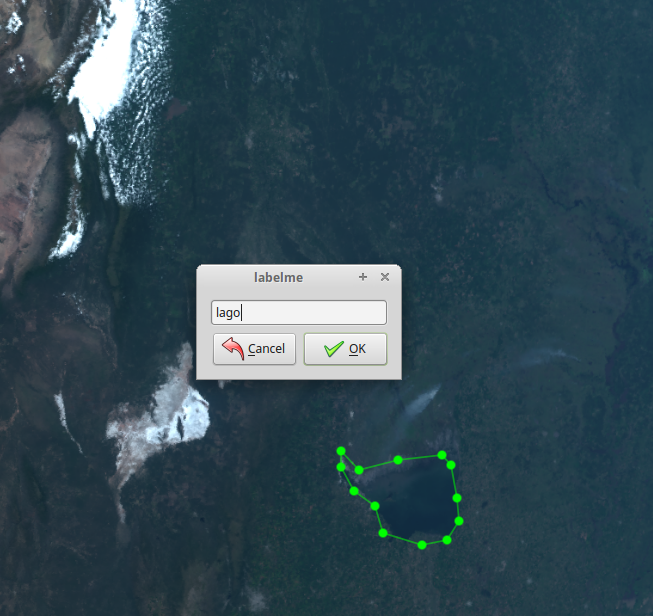
\includegraphics[height=10cm,keepaspectratio=true,clip=true]{imagenes/Logos/labelme2.png}
  \caption{Etiquetar una región en \textit{labelme}}
	\label{Fig: labelme2}
\end{figure}

El \textit{ground truth} final obtenido se guardo en el siguiente formato de anotación (ver \ref{tab:GT} y \ref{tab:ejemGT}):

\begin{table}[H]
\begin{center}
\begin{tabular}{|c|c|c|c|}
\hline Nombre & Bandas & Región & Puntos anotados(x,y)\\ \hline 
\end{tabular}
\end{center} \caption{Estructura ground truth.}\label{tab:GT}
\end{table}

\begin{table}[H]
\begin{center}
\begin{tabular}{|c|c|c|c|}
\hline \textbf{Nombre} & \textbf{Bandas} & \textbf{Región} & \textbf{Puntos anotados(x,y)}\\ \hline 
Imagen01 & 367 & Lago  & 23,50,55,22,223\\ \hline 
Imagen02 & 543 & Lago  & 55,26		\\ \hline 
Imagen03 & 543 & Golfo & 44,300,500,900 \\ \hline 
.......  & ...  & .....& ...............\\ \hline 
\end{tabular}
\end{center} \caption{Ejemplo ground truth.}\label{tab:ejemGT}
\end{table}


\subsection{Regiones Candidatas}\label{sub:proposal}

Cada una de las imágenes obtenidas (ver: \ref{chap:recoleccion}), se aplico técnicas de selección de regiones candidatas para luego ser analizada y clasificada; para esta fase aplicamos métodos de \textit{Regions Proposal} visto en el capitulo \ref{chap:marcoteorico}.

Unos de los principales inconvenientes a la hora del desarrollo de la tesis fue el tamaño de las imágenes. Las regiones de interés son mas pequeñas en proporción a la escala y tamaño de la imagen utilizada, por este motivo al aplicar técnicas de selección de candidatos no generalizaba de manera correcta las regiones que deseamos captar. 

Para eliminar el problema de escala mencionado se procedió a realizar los siguientes pasos: 
\begin{enumerate}
 \item Para cada imagen original se corto en regiones de 256px de alto por el ancho total de la imagen (ver: \ref{Fig: cropimagen}), donde \textit{w} es el ancho de la imagen y \textit{h} alto de la imagen
 \item A cada recorte se aplico técnicas de \textit{Regions Proposal} para la obtención de regiones candidatas (ver: \ref{Fig: cropproposal}).

\begin{figure}[H]
 \centering
  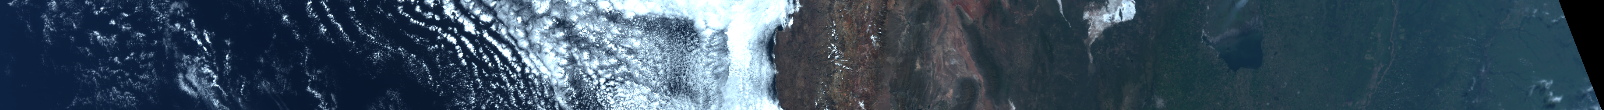
\includegraphics[height=1.2cm,keepaspectratio=true,clip=true]{imagenes/Logos/cropimagen.png}
  \caption{Crop de Imagen Satelital (4833\textit{w} X 256\textit{h})}
	\label{Fig: cropimagen}
\end{figure}

\begin{figure}[H]
 \centering
  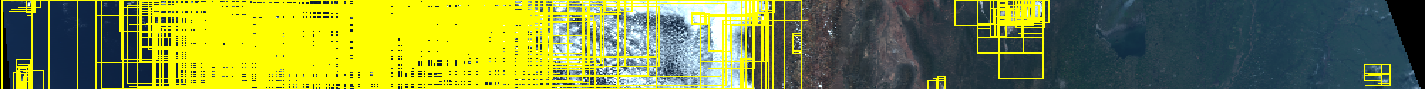
\includegraphics[height=1.1cm,keepaspectratio=true,clip=true]{imagenes/Logos/cropproposal.png}
  \caption{Aplicación de Edges Boxes a un recorte de la imagen.}
	\label{Fig: cropproposal}
\end{figure}

\item Para cada imagen se obtuvo 26 recortes, obteniendo el siguiente resultado en la imagen completa \ref{Fig: proposal}.

\begin{figure}[H]
 \centering
  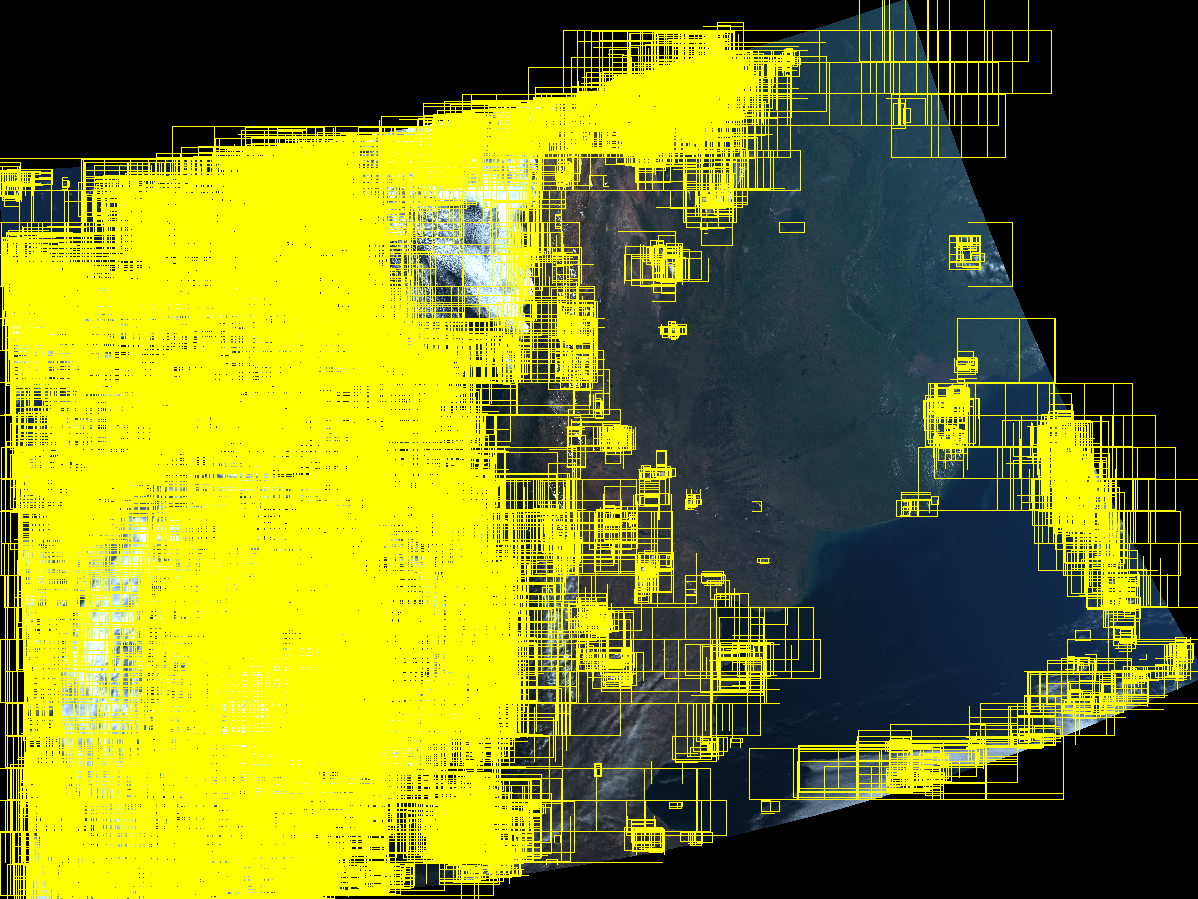
\includegraphics[height=13cm,keepaspectratio=true,clip=true]{imagenes/Logos/proposal.png}
  \caption{Aplicación de Regiones propuestas a una imagen satelital.}
	\label{Fig: proposal}
\end{figure}

\end{enumerate}
La imagen anterior \ref{Fig: proposal} se obtuvo 53.815 regiones por el método \textit{Selective Search} de selección de candidatos. Como se mencionó en \ref{sec:nms} existen regiones solapadas que representan la misma información; esta información fue eliminada aplicando \ac{nms} 

El valor usado para la eliminación de regiones candidatas duplicadas fue de $80\% $ como el porcentaje de solapamiento entre las diferentes regiones candidatas detectadas.

En la figura siguiente \ref{Fig: proposalnms} se pude observar que con un umbral de $80\% $ en \textit{overlapping} aplicando \ac{nms} obtenemos un $90\% $ aproximadamente de optimización en la eliminación de regiones candidatas duplicada, es decir se paso de 53.815 a 1.560 regiones candidatas por imagen para el entrenamiento.

\begin{figure}[H]
 \centering
  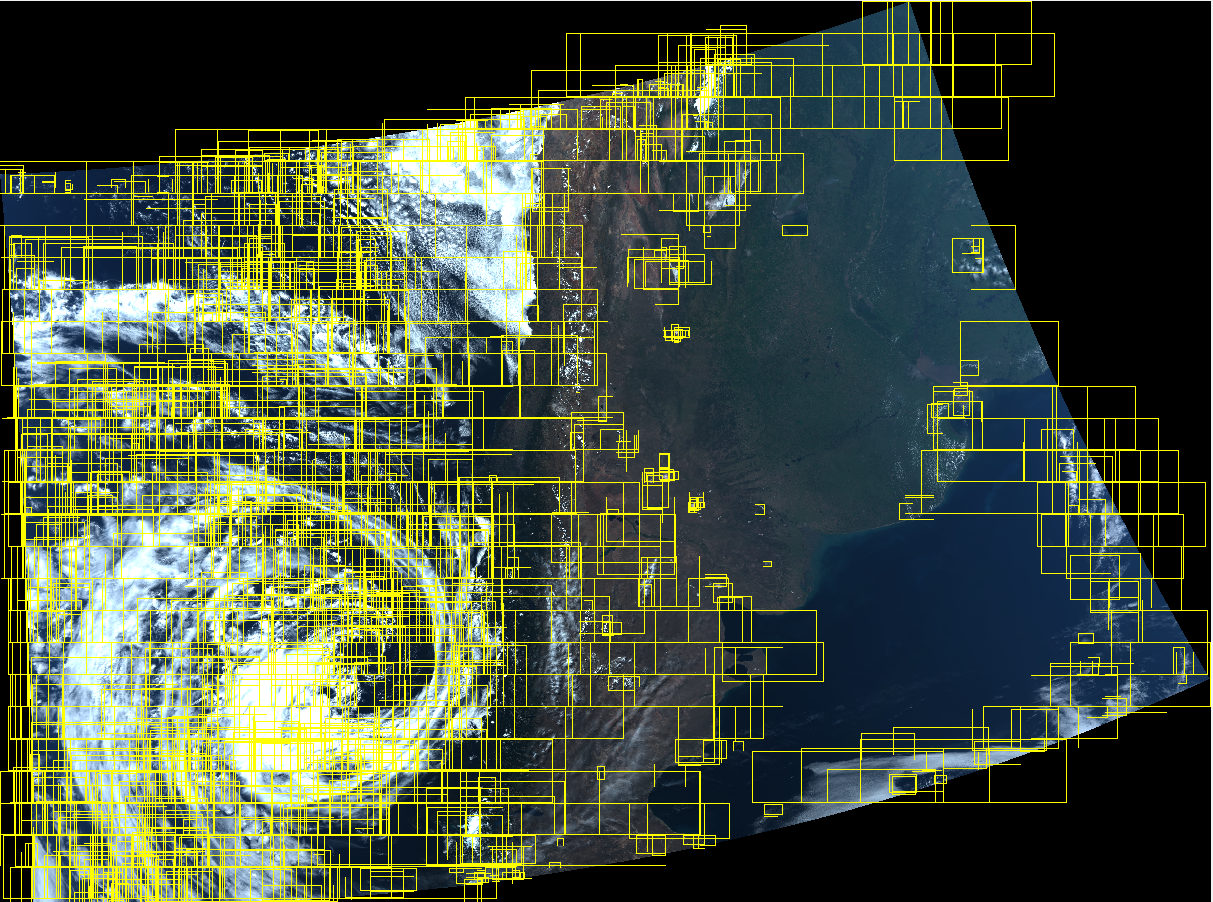
\includegraphics[height=13cm,keepaspectratio=true,clip=true]{imagenes/Logos/proposalconNMS.png}
  \caption{Proposal obtenido con Non-maximum suppression}
	\label{Fig: proposalnms}
\end{figure}


\subsection{Etiquetado}\label{sub:etiquetado}

Los datos obtenidos de la recolección de regiones candidatas a partir de las técnicas de \textit{Regions Propsal} debe ser etiquetados para su entrenamiento. Para realizar el etiquetado se utilizo el \textit{ground truth} \ref{sub:groundtruth} que serán comparados con las regiones candidatas calculando el \textit{overlapping}, solapamiento, entre las regiones.

El criterio utilizado en el etiquetado de datos es el siguiente:
\begin{itemize}
	\item 0: NO contiene el patrón de interés en la región candidata.
	\item 1: Existencia del patrón en la región candidata.
\end{itemize}

Para la selección de alguna de las etiquetas anteriores el umbral de decisión fue de $50\% $ como valor de \textit{overlapping}, esto es el nivel de solapamiento que existen entre el \textit{ground truth} y la región candidata.


\subsection{Extracción de Características}\label{sub:extracciondecaracteristica}

El proceso de extracción de característica se realiza sobre la regiones candidatas obtenidas luego de aplicar \ac{nms} sobre estas. Por cada región se obtendrá un vector de 2048 dimensiones que representa a cada región. La obtención de este vector de característica se realiza por medio de una \ac{cnn}, en donde las entradas a la red son las regiones candidatas. 

Para este proceso se utilizó una red pre-entrenada \textbf{ResNet50}\ref{sec:arquitecturasdered} \ref{chap:pipeline}donde se obtuvo de la ante ultima capa el vector que va a representar la región.

Los vectores obtenidos se almacenaron en un archivo de extensión \textit{.mat}; que contiene los siguientes datos:
\begin{itemize}
 \item Las coordenadas de cada una de las regiones candidatas.
 \item El \textit{feature vector} de 2048 elementos que corresponde a cada región. 
 \item Las etiquetas que indica a que clase pertenece la región \ref{sub:etiquetado}.
\end{itemize}



%%%%% PONER EJEMPLO DE CODIGO???? y crop de las alguno de los regions proposal???


\section{Entrenamiento y Validación}\label{sec:entrenamiento}

En esta sección se comparte como se realizo el proceso de aprendizaje automático \ac{ml} con los datos obtenidos de la sección anterior \ref{sec:preparacion_de_datos}. Luego de la preparación de los datos visto en la sección anterior el conjunto de imágenes finales utilizada para el entrenamiento se detalla en \ref{sec:datosutilizados}.

El datasets final se dividió en tres conjuntos:
\begin{itemize}
\item Train.
\item Test.
\item Validation.
\end{itemize}

El total de la muestra de datos para la experimentación fue de 650.000 \textit{feature vector}.

\subsection{Hiper-parametros}\label{sub:hiperparametro}


Para obtener una predicción correcta se debe realizar la optimización de parámetros que afectan a la clasificación. El método utilizado para poder realizar la optimización de estos parámetros fue \textit{grid search}\footnote{Fuente: https://goo.gl/koWr74}.  Grid search busca por fuerza bruta los parámetros a optimizar quedándose con aquel que logre un mayor \textit{accuracy} en las evaluaciones; en cada iteración se utiliza \textit{cross-validation} con 5 folds en el entrenamiento para evitar el \textit{overfitting}.

Los parametros son:
\begin{enumerate}
	\item \textbf{Parámetro C}: Controla el costo de la mala clasificación, \textit{misclassification}, en los datos de entrenamiento. Con un valor de C pequeño hará que el optimizador busque un hiperplano de separación de mayor margen, incluso si ese hiperplano clasifica erróneamente más puntos. Para valores muy pequeños de C, debe obtener ejemplos mal clasificados, a menudo incluso si sus datos de entrenamiento son linealmente separables. Para valores grandes de C,  elegirá un hiperplano de menor margen si ese hiperplano hace un mejor trabajo de conseguir que todos los puntos de entrenamiento estén clasificados correctamente. El objetivo es encontrar el equilibrio entre "no demasiado estricto" y "no demasiado relajado". La validación cruzada  son buenas maneras de encontrar el mejor C.
	\item \textbf{Parámetro gamma}: Es la inversa de la desviación estándar del kernel RBF (función gaussiana), que se utiliza como medida de similitud entre dos puntos.
\end{enumerate}
	

El rango de parámetros usados para el entrenamiento y validación de datos fueron los siguientes:

\begin{itemize}
 \item \textbf{Valor de C}: 1000,100,10,1, 0.1,0.01,0.001,0.0001
 \item \textbf{Valor de Gamma}: 1,0,1,0,01,0,001,0,0001,0,00001
\end{itemize}




\subsection{Metricas}\label{sub:metricas}

Además de la optimización de los parámetros mencionados \ref{sub:hiperparametro}, la validación de los resultados se usaron las siguientes métricas: \textit{Accuracy, Precisión y Recall}.

\begin{itemize}
	\item Positivos (P): Observación positiva (valor etiquetado).
	\item Verdadero Positivo (TP): La observación es positiva y la predicción también.
	\item Falso Negativo (FN): La observación es positiva pero la predicción es negativa.
	\item Falso Positivo (FP): La observación es negativa pero la predicción es positiva.
	\item Verdadero Negativo (TN) :  La observación es negativa y también la predicción negativa.
\end{itemize}

\begin{enumerate}
\item \textbf{Accuracy:} Proporción de todas las predicciones que son correctas; da una medida de que tan bueno es el modelo.
\begin{equation}
accuracy = \frac{FP+FN}{FP+FN+TP+TN}=\frac{predicciones\;correctas}{todas\;las\;predicciones}
\end{equation}

\item \textbf{Precisión:} Proporción de todas las predicciones positivas que son correctas. La precisión es una medida de cuántas predicciones positivas son reales.
\begin{equation}
precision=\frac{TP}{TP+FP}= \frac{predicciones\;correctamente\;positivas}{todas\;las\;predicciones\;positivas}
\end{equation}

\item \textbf{Recall:} Nos da la proporción de la observaciones reales positivas que son correcta, es decir nos da la precisión de cuantas observaciones positivas reales se obtuvo correctamente.
\begin{equation}
recall = \frac{TP}{TP+FN} = \frac{TP}{P} = \frac{predicciones\;a\;ser\;positiva}{todas\;la\;observaciones\;positivas} 
\end{equation}

\item \textbf{Overlapping Mean:} Métrica obtenida a partir de la intersección del ground truth y el bounding box de la predicción obtenida.

\end{enumerate}


\subsection{Resultados obtenidos}\label{sub:resultados}

En la siguiente tabla \ref{tab:entrenam-result}	se expone los resultados obtenidos de los entrenamientos realizados. Como podemos ver se consideraron  diferentes combinaciones de banda con el fin de encontrar aquella que mejoren las métricas y que resalten las zonas de interés que deseamos detectar.

\begin{table}[H]
\begin{center}
\begin{tabular}{|c|c|c|c|c|c|c|c|}
\hline
 & \multicolumn{3}{c|}{Hiper - parametros} & \multicolumn{4}{c|}{Metricas} \\ \hline
Bandas & C & gamma & kernel & precision & recall & \begin{tabular}[c]{@{}c@{}}average\\ presicion\end{tabular} & \begin{tabular}[c]{@{}c@{}}overlapping\\ mean\end{tabular} \\ \hline
\multicolumn{1}{|c|}{1-1-1} & 10 & - & linear & 0.91 & 0.91 & 0.18 & 0.1 \\ \hline
\multicolumn{1}{|c|}{1-3-5} & 10 & - & linear & 0.93 & 0.94 & 0.57 & 0.28 \\ \hline
\multicolumn{1}{|c|}{1-5-3} & 1000 & 0.01 & rbf & 0.94 & 0.94 & 0.61 & 0.27 \\ \hline
\multicolumn{1}{|c|}{3-1-5} & 100 & 0.01 & rbf & 0.93 & 0.94 & 0.61 & 0.31 \\ \hline
\multicolumn{1}{|c|}{3-3-3} & 1000 & 1 & rbf & 0.92 & 0.92 & 0.28 & 0.1 \\ \hline
\multicolumn{1}{|c|}{3-5-1} & 10 & 0.01 & rbf & 0.90 & 0.91 & 0.66 & 0.25 \\ \hline
\multicolumn{1}{|c|}{5-1-3} & 1 & 1 & rbf & 0.89 & 0.86 & 0.46 & 0.29 \\ \hline
\multicolumn{1}{|c|}{5-3-1} & 1000 & 0.001 & rbf & 0.90 & 0.88 & 0.38 & 0.21 \\ \hline
\multicolumn{1}{|c|}{5-5-5} & 100 & 0.01 & rbf & 0.89 & 0.85 & 0.63 & 0.26 \\ \hline
\multicolumn{1}{|c|}{7-7-7} & 1000 & 0.001 & rbf & 0.92 & 0.92 & 0.75 & 0.30 \\ \hline
\multicolumn{1}{|c|}{9-9-9} & 10 & 1 & rbf & 0.82 & 0.75 & 0.34 & 0.1 \\ \hline
\multicolumn{1}{|c|}{11-7-9} & 1000 & 0.001 & rbf & 0.91 & 0.86 & 0.59 & 0.24 \\ \hline
\multicolumn{1}{|c|}{11-9-7} & 10 & - & linear & 0.91 & 0.89 & 0.74 & 0.26 \\ \hline
\multicolumn{1}{|c|}{7-11-9} & 1 & 1 & rbf & 0.91 & 0.87 & 0.60 & 0.27 \\ \hline
\multicolumn{1}{|c|}{7-9-11} & 10 & - & linear & 0.90 & 0.89 & 0.73 & 0.28 \\ \hline
\multicolumn{1}{|c|}{9-11-7} & 1 & 1 & rbf & 0.89 & 0.86 & 0.66 & 0.23 \\ \hline
\multicolumn{1}{|c|}{9-7-11} & 1 & 1 & rbf & 0.89 & 0.86 & 0.79 & 0.30 \\ \hline
\multicolumn{1}{|c|}{11-11-11} & 1 & 1 & rbf & 0.91 & 0.88 & 0.74 & 0.27 \\ \hline
\multicolumn{1}{|c|}{11-3-15} & 10 & 0.1 & rbf & 0.89 & 0.83 & 0.59 & 0.3 \\ \hline
\multicolumn{1}{|c|}{11-15-13} & 1 & 1 & rbf & 0.89 & 0.84 & 0.63 & 0.28 \\ \hline
\multicolumn{1}{|c|}{13-11-15} & 10 & - & linear & 0.89 & 0.87 & 0.61 & 0.26 \\ \hline
\multicolumn{1}{|c|}{13-13-13} & 1 & - & linear & 0.91 & 0.90 & 0.32 & 0.35 \\ \hline
\multicolumn{1}{|c|}{13-15-11} & 1 & - & linear & 0.89 & 0.82 & 0.39 & 0.26 \\ \hline
\multicolumn{1}{|c|}{15-11-13} & 10 & 1 & rbf & 0.89 & 0.86 & 0.51 & 0.25 \\ \hline
\multicolumn{1}{|c|}{15-13-11} & 1000 & 0.001 & rbf & 0.90 & 0.86 & 0.54 & 0.27 \\ \hline
\multicolumn{1}{|c|}{15-15-15} & 10 & 1 & rbf & 0.88 & 0.85 & 0.26 & 0.28 \\ \hline
\multicolumn{1}{|c|}{11-12-13} & 1000 & 1 & rbf & 0.87 & 0.91 & 0.62 & 0.32 \\ \hline
\multicolumn{1}{|c|}{5-4-3} & 1000 & 1 & rbf & 0.88 & 0.87 & 0.57 & 0.27 \\ \hline
\multicolumn{1}{|c|}{10-7-5} & 1000 & 0.001 & rbf & 0.91 & 0.96 & 0.58 & 0.36 \\ \hline
\end{tabular}
\end{center}\caption{Resultados de los entrenamientos}\label{tab:entrenam-result}
\end{table}

Cada uno de los valores encontrados de los hiper parámetros se obtuvo a través de \textit{grid search}, estos valores son los que optimizan las métricas que estamos empleando.

Se evaluaron también las detecciones obtenidas en el conjunto de test evaluando los \textit{falsos positivos} y re entrenando nuevamente el clasificador con los falsos positivos obtenidos con el fin de lograr una mejora en la detección y localización de las regiones que estamos buscando.

Las tareas realizadas para evaluar la localización del objeto fue obtener el \textit{overlapping mean}; en esta métrica comparamos los \textit{bounding boxs} obtenidos en el entrenamiento realizado y el \textit{ground thruth}, región de interés, que tenemos anotado. Este valor nos da una visión de cual es la exactitud de nuestro predictor en cuanto a la localización del objeto.

En el siguiente cuadro se visualiza la relación existente entre las regiones detectado y la presicion de la detección \ref{Fig: trade-off}.


\begin{figure}[H]
 \centering
  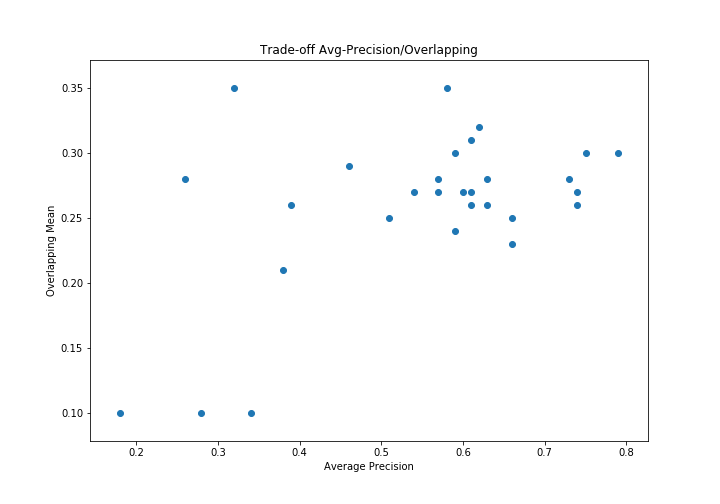
\includegraphics[height=9cm,keepaspectratio=true,clip=true]{imagenes/Evaluacion-exp/presicion-over.png}
  \caption{Trade-Off Average Presicion-Overlapping}
	\label{Fig: trade-off}
\end{figure}

La siguiente imagen se puede visualizar los \textit{bounding boxs} detectados, esto es el resultado de aplicar el modelo entrenado a una imagen satelital; en este caso la imagen utilizada pertenece a las bandas M9-M7-M11, como se puede ver en la tabla \ref{tab:entrenam-result}, esta combinación de banda es una de las que mejores métricas se obtuvo en términos de localización y presicion en los entrenamientos.


\begin{figure}[H]
 \centering
  \includegraphics[height=9cm,keepaspectratio=true,clip=true]{imagenes/Evaluacion-exp/prediction-9711.png}
  \caption{Ejemplo de predicciones positivas}
	\label{Fig: TP}
\end{figure}
